%---------------------导言区---------------------------%
\documentclass[12pt,a4paper,UTF8]{ctexart}
	%10pt:正文字体为12pt,缺省为10pt;各层级字体大小会根据正文字体自动调整
	%a4paper:纸张大小a4;
	%UTF8:中文要求
%\usepackage{syntonly}
%\syntaxonly%加快编译速度
\usepackage{geometry}%用于设置上下左右页边距
	\geometry{left=2.5cm,right=2.5cm,top=3.2cm,bottom=2.8cm}
\usepackage{xeCJK,amsmath,paralist,enumerate,booktabs,multirow,graphicx,float,subfig,setspace,listings,lastpage,hyperref,gensymb}
	%xeCJK:中文字体(如楷体,作者和机构需要用到)的设置
	%amsmath:数学公式
	%paralist,enumerate:自定义项目符号
	%booktabs:三线图,论文常用的表格风格
	%multirow:复杂表格
	%graphicx,float: 插入图片
	%subfig:并排排版图片以及强制图表显示在“这里”[H]
	%setspace:设置行间距等功能
	\setlength{\parindent}{2em}%正文首行缩进两个汉字
	%listings:用于排版各种代码;比如matlab的代码
	%\lstset{language=Matlab}%matlab代码
	%lastpage:获取总页数;
	%hyperref:超链接,和lastpage搭配.
\usepackage{fancyhdr}
	%fancyhdr:一个很强大的宏包,用于自定义设计页面风格并命名以供调用。
	\pagestyle{fancy}
	\rhead{实验十八~弗兰克-赫兹实验}
	\lhead{普通物理实验\uppercase\expandafter{\romannumeral1}实验报告}
	\cfoot{\thepage}  
		%分别是右页眉、左页眉、右页脚
	\renewcommand{\headrulewidth}{0.4pt}
	\renewcommand{\theenumi}{(\arabic{enumi})}

\setCJKmainfont{FZSSK.TTF}[ItalicFont=FZKTK.TTF, BoldFont=FZHTK.TTF]
%中文字体设置:使用开源字体方正书宋,方正楷体和方正黑体



%%%%%%%%%%%%%%%%%%%%%%%%%%%%%%%%%%%%%%%%%%%%%%%%%%%%%%%%%%
%%%%%%%%%%%%%%%%%%%%%%%%%正文开始%%%%%%%%%%%%%%%%%%%%%%%%%%
%%%%%%%%%%%%%%%%%%%%%%%%%%%%%%%%%%%%%%%%%%%%%%%%%%%%%%%%%%

\begin{document}

%%begin-------------------标题与信息-----------------------%%

%%标题
\begin{center}
\LARGE\textbf{实验十八~弗兰克-赫兹实验}
\end{center}

%%信息
\begin{doublespacing}
	%doublespacing:手动两倍行距
	\centering
	\begin{tabular}{lr}
	 & \\
	{\CJKfontspec{STKAITI.TTF} 实验人:钟易轩(2000012706)} \\
	{\CJKfontspec{STKAITI.TTF} 组号:九组七号} & {\CJKfontspec{STKAITI.TTF}指导教师:陈志忠}\\
	{\CJKfontspec{STKAITI.TTF} 实验时间:2021年11月5日~星期五~下午} &{\CJKfontspec{STKAITI.TTF} 实验地点:物理楼南楼~225}
	\end{tabular}
\end{doublespacing}

%%end-------------------标题与信息-----------------------%%

\subsection*{【实验目的】}
	\begin{enumerate}[(1)]
		\item 了解弗兰克-赫兹用伏安法证明原子存在能级的原理和方法
		\item 学习用伏安法测量非线性器件
		\item 学习微电流的测量
	\end{enumerate}
	
\subsection*{【仪器用具】}
	\paragraph{弗兰克-赫兹管(充汞和充氩两种),F-H管电源,扫描电源和微电流放大器.}
	
\subsection*{【实验数据及处理】}

\subsubsection*{1.汞管实验注意事项及数据}
	
	\begin{enumerate}[(1)]
	\item 待管温稳定之后,调节$U_F$、$U_{g_2p}$时,每次调节$0.1V$,至少等3到5分钟.
	\item 细测时,$U_{kg_2}$取点间隔在峰值附近$0.1V$左右,在其他位置$0.3V$左右.
	\end{enumerate}
	\par
	实验条件:
	$U_F=2.1V\qquad	U_{g_{2}p}=2.0V\qquad \theta=177\degree C$ 
	\par
	粗测数据如下:
	\begin{table}[htbp]	
	\centering
	\scalebox{1.2}{
	\begin{tabular}{|c|c|c|c|c|c|c|}
	\hline
	$U_{kg_2}/V$&4.6&9.1&13.9&18.8&23.9&28.8 \\
	\hline
	$U_{out}/V$&0.043&0.084&0.123&0.169&0.184&0.222 \\
	\hline
	\end{tabular}}
	\end{table}
	\newpage
	细测数据如下:
	\begin{table}[htbp]
	\centering
	\scalebox{1.2}{
	\begin{tabular}{|c|c||c|c||c|c||c|c|}
\hline
      $U_{kg_2}/V$&       $U_{out}/V$ &     $U_{kg_2}/V$ &     $U_{out}/V$ &      $U_{kg_2}/V$ &    $U_{out}/V$ &     $U_{kg_2}/V$ &     $U_{out}/V$ \\
\hline
       0.4 &      0.025 &          \textbf{9.0} &      \textbf{0.089} &       15.6 &      0.042 &       23.2 &      0.182 \\
\hline
       0.7 &      0.026 &        9.1 &      0.088 &       15.9 &      0.041 &       23.4 &      0.201 \\
\hline
       1.2 &      0.026 &        9.2 &      0.084 &       16.3 &      0.046 &       23.5 &      0.202 \\
\hline
       1.7 &      0.027 &        9.4 &      0.067 &       16.6 &       0.050 &       23.7 &      0.204 \\
\hline
       2.3 &      0.028 &        9.7 &      0.052 &         17.0 &      0.062 &       \textbf{23.8} &       \textbf{0.210} \\
\hline
       2.8 &       0.030 &         10.0 &      0.046 &       17.3 &      0.077 &         24.0 &      0.205 \\
\hline
       3.3 &      0.034 &       10.3 &      0.041 &       17.6 &      0.092 &       24.3 &      0.178 \\
\hline
       3.8 &      0.034 &       10.6 &      0.038 &       17.9 &      0.105 &       24.5 &      0.167 \\
\hline
       4.2 &      0.038 &       10.9 &      0.037 &       18.2 &      0.125 &       24.9 &      0.122 \\
\hline
       4.4 &      0.038 &       11.2 &      0.038 &       18.4 &      0.142 &       25.2 &      0.095 \\
\hline
       4.5 &      0.039 &       11.5 &      0.041 &       \textbf{18.6} &      \textbf{0.156} &       25.4 &      0.079 \\
\hline
       \textbf{4.6} &     \textbf{0.039} &       11.9 &      0.047 &       18.8 &      0.155 &       25.9 &      0.069 \\
\hline
       4.7 &      0.037 &       12.3 &      0.058 &       18.9 &      0.152 &       26.2 &       0.070 \\
\hline
       4.8 &      0.037 &       12.6 &       0.070 &         19.0 &      0.148 &       26.5 &      0.076 \\
\hline
       4.9 &      0.036 &       12.9 &      0.082 &       19.4 &       0.110 &       26.8 &      0.091 \\
\hline
       5.0 &      0.035 &       13.3 &        0.100 &       19.8 &      0.083 &       27.1 &      0.104 \\
\hline
       5.6 &      0.033 &       13.5 &      0.115 &       20.1 &      0.068 &       27.4 &      0.127 \\
\hline
       6.0 &      0.032 &       13.7 &      0.122 &       20.4 &      0.054 &       27.7 &       0.160 \\
\hline
       6.4 &      0.031 &       \textbf{13.8} &      \textbf{0.125} &       20.7 &      0.051 &       28.1 &      0.203 \\
\hline
       6.8 &      0.036 &       13.9 &      0.118 &       21.1 &      0.052 &       28.5 &      0.237 \\
\hline
       7.2 &       0.040 &         14.0 &      0.116 &       21.4 &      0.057 &       28.6 &      0.238 \\
\hline
       7.7 &      0.049 &       14.2 &      0.102 &       21.9 &      0.076 &       \textbf{28.9} &      \textbf{0.242} \\
\hline
       8.1 &       0.060 &       14.5 &      0.077 &       22.2 &      0.092 &       29.1 &       0.240 \\
\hline
       8.6 &      0.076 &       14.8 &       0.060&       22.5 &      0.112 &       29.3 &      0.222 \\
\hline
       8.9 &      0.087 &       15.1 &       0.050 &       22.8 &      0.143 &            &            \\
\hline
\end{tabular} }
\end{table} 
\newpage
经matlab画出如下图像:
\begin{figure}[htb]
\center{
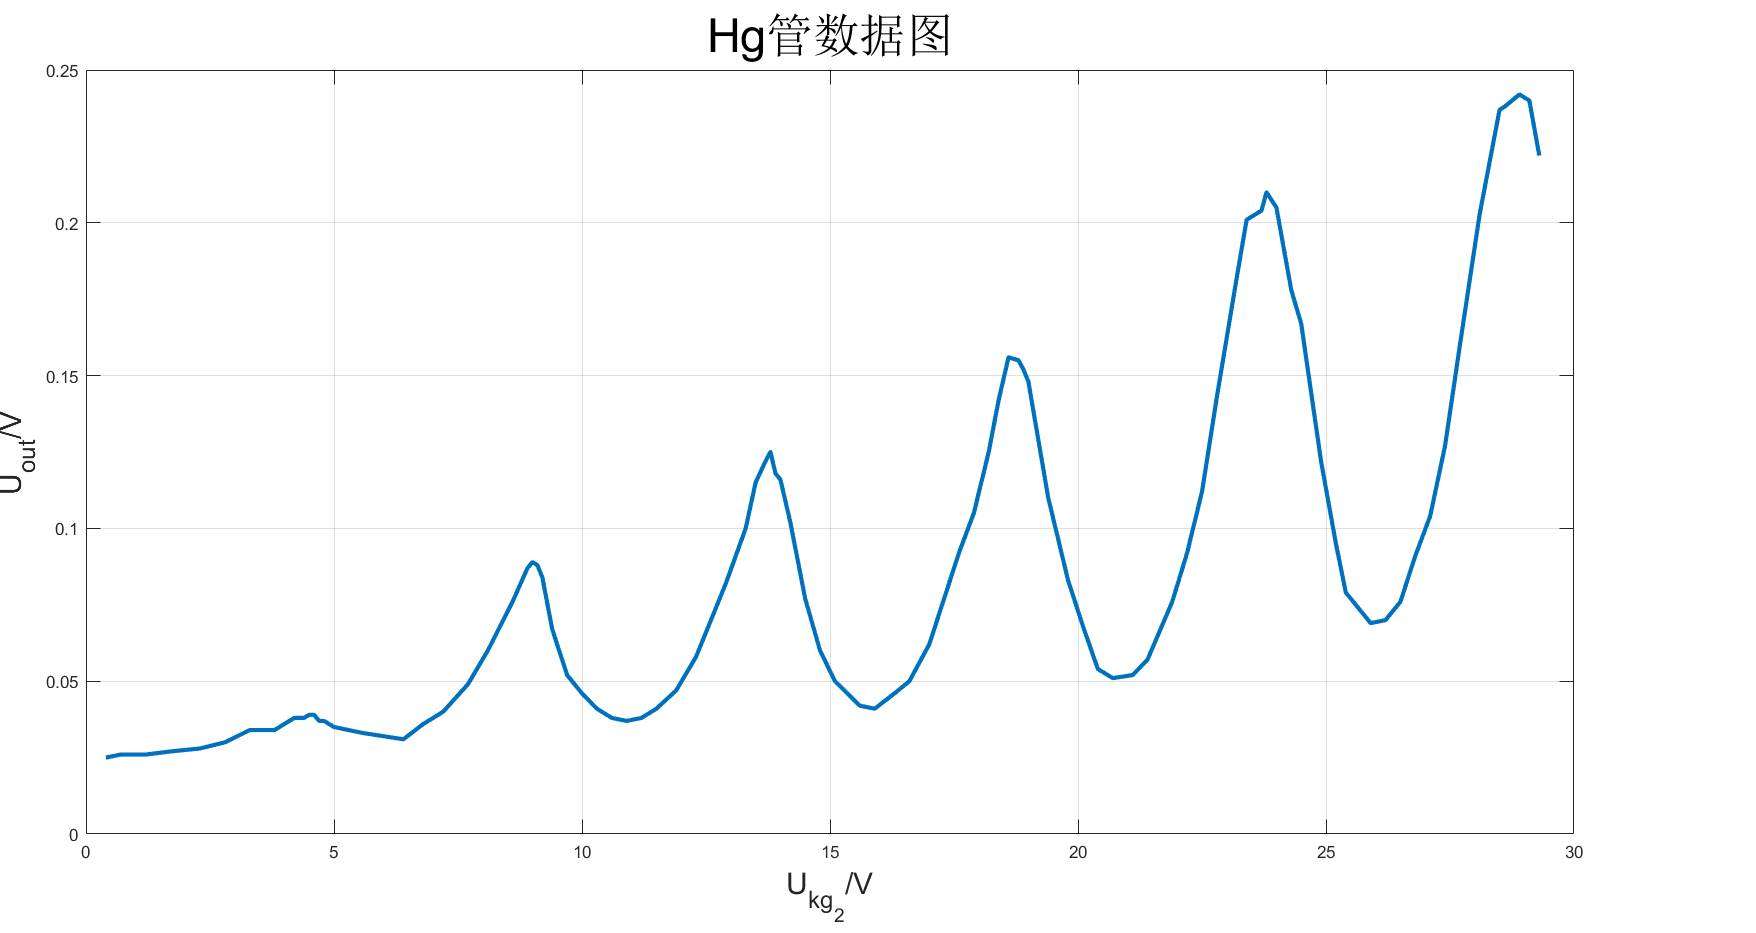
\includegraphics[width=18cm]{Hgtube.png}}
\end{figure}

\subsubsection*{2.Ar管实验注意事项及数据}
\begin{enumerate}[(1)]
	\item 待管温稳定之后,调节$U_F、U_{g_2p}$时,每次调节$0.1V$,至少等3到5分钟.
	\item 细测时,$U_{kg_2}$取点间隔在峰值附近$0.2V$左右,在其他位置$0.5V$左右.
	\end{enumerate}
	\par
	实验条件:
	$U_F=2.2V\qquad	U_{g_1g_2}=6.1V\qquad U_{g_{2}p}=2.0V\qquad $ 
	\par
	粗测数据如下:
	\begin{table}[htbp]	
	\centering
	\scalebox{1.2}{
	\begin{tabular}{|c|c|c|c|c|c|c|}
	\hline
	$U_{kg_2}/V$&16.4&27.7&40.3&52.6&65.5&79.0 \\
	\hline
	$I/nA$&22.1&39.1&50.5&61.3&74.6&94.5 \\
	\hline
	\end{tabular}}
	\end{table}
	~\\
	\par
	细测数据如下:
\begin{table}[htbp]
	\centering
	\scalebox{1.1}{
\begin{tabular}{|c|c||c|c||c|c||c|c|}
\hline
         $U_{kg_2}/V$ &        $I/nA$ &    $U_{kg_2}/V$ &   $I/nA$&  $U_{kg_2}/V$ &    $I/nA$ &   $U_{kg_2}/V$ &   $I/nA$ \\
\hline
      7.9  &       0.1  &      27.5  &      36.3  &      47.0  &      24.3  &\textbf{65.0}  &\textbf{77.7}  \\
\hline
      8.5  &       1.5  &      27.9  &      36.2  &      47.7  &      33.9  &      65.2  &      77.5  \\
\hline
      9.0  &       3.1  &      28.5  &      35.1  &      48.1  &      38.2  &      65.3  &      77.3  \\
\hline
      9.5  &       6.4  &      29.2  &      32.6  &      48.7  &      44.8  &      65.5  &      77.0  \\
\hline
     10.0  &      11.0  &      29.8  &      29.3  &      49.0  &      47.8  &      66.0  &      75.8  \\
\hline
     10.7  &      15.5  &      30.5  &      23.3  &      49.3  &      51.0  &      66.6  &      72.8  \\
\hline
     11.1  &      18.0  &      31.0  &      17.9  &      49.7  &      53.8  &      67.2  &      69.8  \\
\hline
     11.6  &      19.7  &      31.5  &      12.9  &      50.0  &      55.7  &      67.7  &      64.6  \\
\hline
     12.1  &      20.7  &      32.0  &       9.1  &      50.5  &      58.1  &      68.3  &      58.5  \\
\hline
     12.7  &      22.2  &      32.6  &       5.6  &      50.8  &      59.5  &      68.8  &      54.2  \\
\hline
     13.3  &      23.1  &      33.1  &       4.0  &      51.1  &      60.7  &      69.3  &      50.8  \\
\hline
     13.8  &      23.3  &      33.5  &       3.7  &      51.5  &      61.8  &      69.8  &      48.0  \\
\hline
     \textbf{14.0}  &      \textbf{23.3}  &      34.2  &       6.6  &      51.7  &      62.2  &      70.6  &      47.4  \\
\hline
     14.1  &      22.6  &      34.7  &      12.7  &      51.9  &      62.7  &      71.0  &      48.9  \\
\hline
     14.2  &      22.3  &      35.3  &      20.2  & \textbf{52.1}  & \textbf{62.7}  &      71.5  &      51.4  \\
\hline
     14.8  &      22.1  &      35.8  &      27.6  &      52.3  &      62.6  &      72.0  &      54.4  \\
\hline
     15.2  &      22.0  &      36.3  &      33.4  &      52.5  &      62.3  &      72.6  &      59.0  \\
\hline
     15.8  &      22.0  &      36.8  &      37.7  &      53.0  &      61.1  &      73.2  &      63.9  \\
\hline
     16.3  &      22.1  &      37.3  &      41.6  &      53.5  &      58.3  &      73.8  &      69.2  \\
\hline
     16.8  &      21.7  &      37.8  &      45.0  &      54.0  &      55.0  &      74.4  &      75.3  \\
\hline
     17.3  &      20.9  &      38.3  &      47.0  &      54.7  &      49.0  &      75.1  &      81.1  \\
\hline
     17.8  &      19.7  &      38.8  &      48.2  &      55.1  &      44.6  &      75.4  &      83.3  \\
\hline
     18.4  &      17.5  & \textbf{39.3}  & \textbf{49.0}  &      55.8  &      36.4  &      75.9  &      86.8  \\
\hline
     19.0  &      15.4  &      39.5  &      48.8  &      56.3  &      31.0  &      76.5  &      90.3  \\
\hline
     19.5  &      12.8  &      39.6  &      48.8  &      56.8  &      25.8  &      77.0  &      93.3  \\
\hline
     20.0  &      10.1  &      39.8  &      48.8  &      57.3  &      23.2  &      77.3  &      94.3  \\
\hline
     20.6  &       7.7  &      40.0  &      48.6  &      57.9  &      24.5  &      77.5  &      94.9  \\
\hline
     21.2  &       6.0  &      40.3  &      48.4  &      58.4  &      27.6  &      77.6  &      95.3  \\
\hline
     21.8  &       4.7  &      40.5  &      47.8  &      58.9  &      31.7  &      77.8  &      95.9  \\
\hline
     22.4  &       5.6  &      41.0  &      45.7  &      59.4  &      37.1  &      77.9  &      96.3  \\
\hline
     23.0  &       9.2  &      41.5  &      42.4  &      60.1  &      44.7  &      78.2  &      96.7  \\
\hline
     23.6  &      15.2  &      42.0  &      38.7  &      60.6  &      50.4  &      78.5  &      97.3  \\
\hline
     24.2  &      21.0  &      42.5  &      33.9  &      61.2  &      56.2  &      78.7  &      97.3  \\
\hline
     24.8  &      26.8  &      43.0  &      28.2  &      61.8  &      61.5  &\textbf{78.8}  &\textbf{97.3}  \\
\hline
     25.5  &      31.9  &      43.5  &      21.4  &      62.3  &      66.5  &      79.0  &      97.0  \\
\hline
     26.0  &      34.1  &      44.0  &      15.6  &      62.9  &      70.6  &      79.3  &      96.7  \\
\hline
     26.5  &      35.5  &      44.6  &      10.9  &      63.4  &      72.7  &      79.5  &      96.0  \\
\hline
     27.0  &      36.4  &      45.0  &       8.5  &      63.7  &      74.2  &      80.1  &      93.3  \\
\hline
     \textbf{27.1}  &      \textbf{36.5}  &      45.5  &       8.6  &      63.9  &      75.0  &            &            \\
\hline
     27.2  &      36.4  &      46.0  &      12.2  &      64.3  &      75.9  &            &            \\
\hline
     27.4  &      36.4  &      46.5  &      18.3  &      64.7  &      76.9  &            &            \\
\hline
\end{tabular}  }
\end{table}
\newpage
经matlab画出如下图像:
\begin{figure}[htb]
\center{
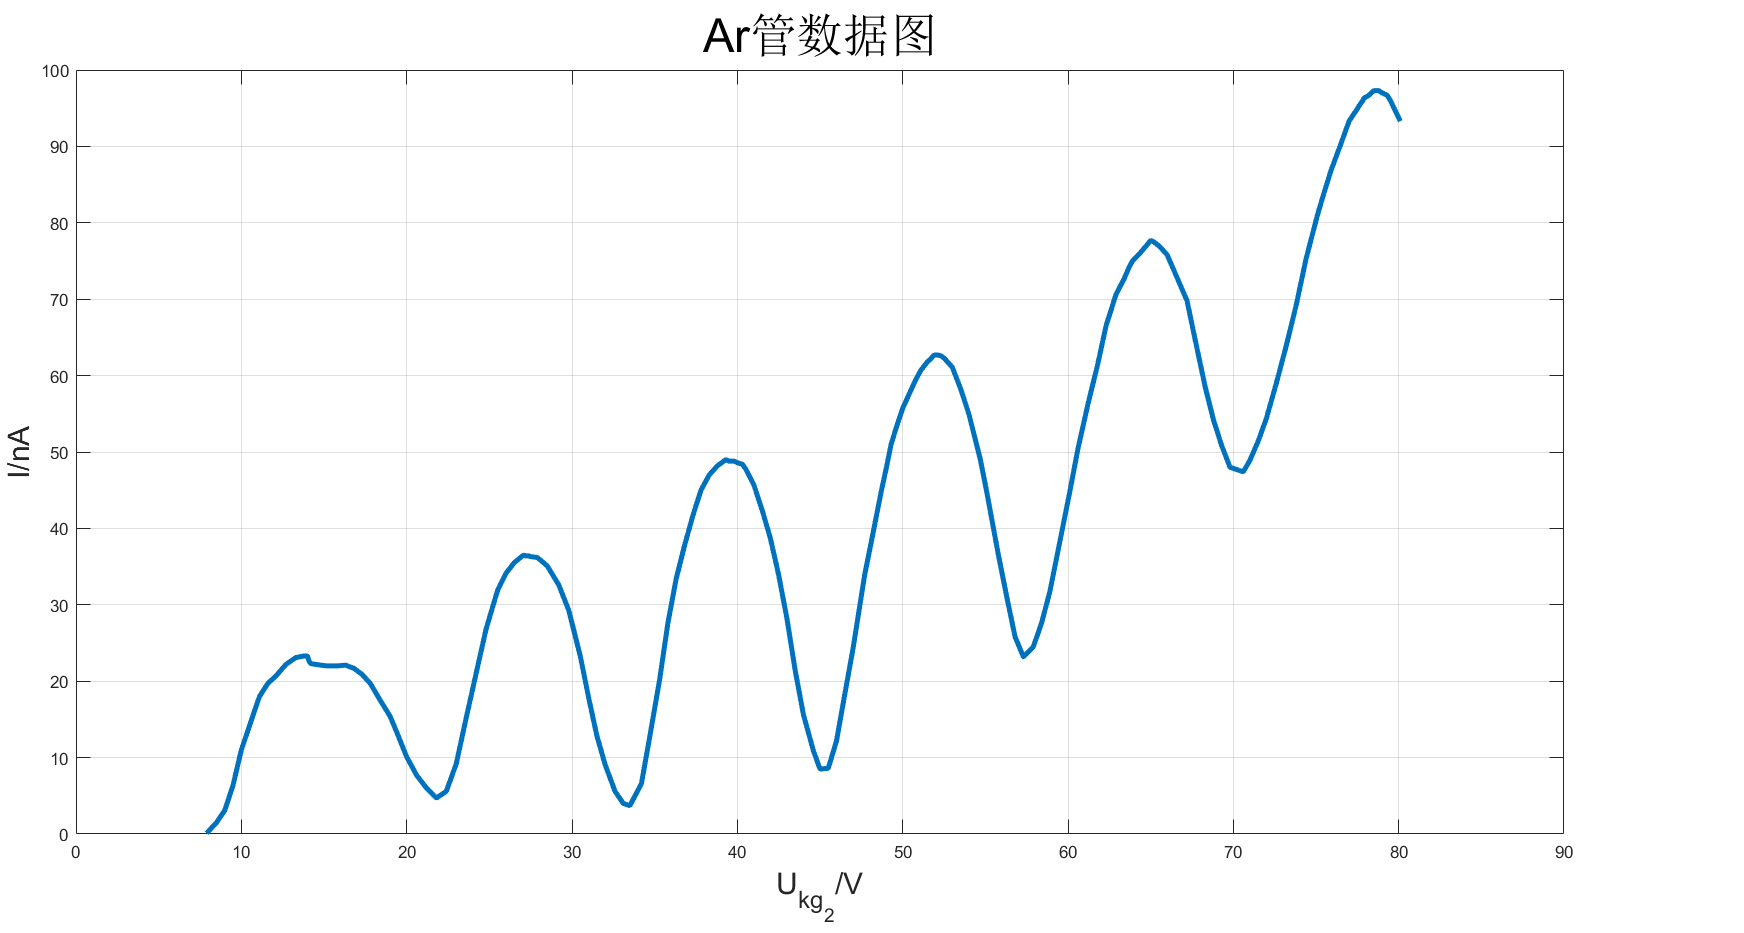
\includegraphics[width=18cm]{Artube.png}}
\end{figure}
\subsubsection*{3.Hg管改变$U_{g_2p}$之后的数据}	

\textcircled{1}当$U_{g_2p}=0.89V$且其余数据未变情况下,数据表如下:
\begin{table}[htbp]
\centering
\scalebox{1.2}{

\begin{tabular}{|c|c||c|c||c|c||c|c|}
\hline
       $U_{kg_2}/V$ & $U_{out}/V$ &  $U_{kg_2}/V$ & $U_{out}/V$  & $U_{kg_2}/V$ & $U_{out}/V$  &  $U_{kg_2}/V$ & $U_{out}/V$  \\
\hline
      22.4 &      0.204 &\textbf{23.7}&\textbf{0.301} &       25.6 &      0.111 &       28.1 &      0.339 \\
\hline
      22.6 &      0.211 &       23.8 &      0.298 &         26 &      0.118 &       28.3 &      0.359 \\
\hline
      22.9 &      0.245 &       23.9 &      0.285 &       26.4 &      0.142 &       28.4 &      0.374 \\
\hline
      23.2 &      0.267 &       24.3 &      0.216 &       26.8 &      0.172 &\textbf{28.6} &\textbf{0.378} \\
\hline
      23.3 &      0.281 &       24.5 &      0.191 &       27.1 &      0.208 &       28.7 &      0.364 \\
\hline
      23.4 &      0.291 &       24.7 &      0.161 &       27.3 &      0.232 &       28.9 &      0.362 \\
\hline
      23.5 &      0.299 &         25 &      0.129 &       27.7 &      0.282 &            &            \\
\hline
      23.6 &      0.299 &       25.3 &      0.116 &       27.9 &      0.309 &            &            \\
\hline
\end{tabular}  }
\end{table}
\newpage
经matlab画出如下图像:
\begin{figure}[htbp]
\center{
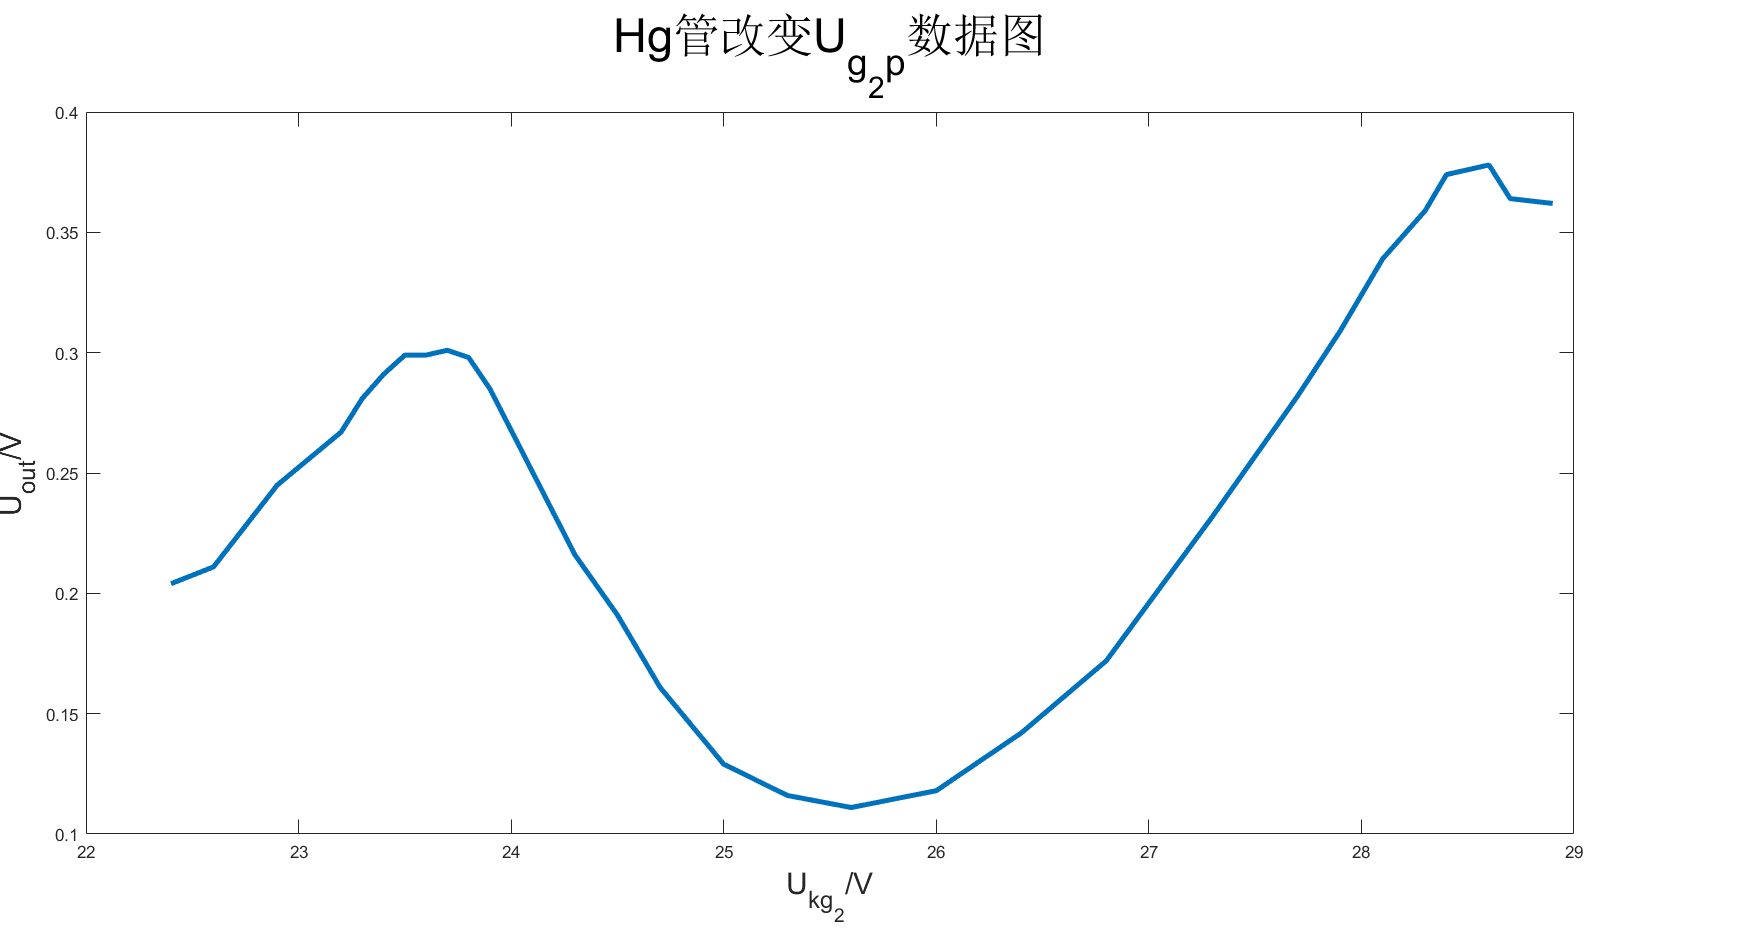
\includegraphics[width=18cm]{Hg0.89.png}}
\end{figure}
\par
\textcircled{2}当$U_{g_2p}=2.92V$且其余条件未变情况下,数据表如下:
\begin{table}[htbp]
\centering
\scalebox{1.2}{
\begin{tabular}{|c|c||c|c||c|c||c|c|}
\hline
       $U_{kg_2}/V$ & $U_{out}/V$ &  $U_{kg_2}/V$ & $U_{out}/V$  & $U_{kg_2}/V$ & $U_{out}/V$  &  $U_{kg_2}/V$ & $U_{out}/V$  \\
\hline
        22 &      0.047 &         24 &      0.124 &       26.5 &      0.052 &       28.7 &      0.127 \\
\hline
      22.4 &      0.055 &       24.1 &      0.124 &       26.8 &      0.051 &       28.8 &      0.128 \\
\hline
      22.8 &      0.072 &       24.5 &      0.109 &       27.1 &      0.058 &\textbf{28.9} &\textbf{0.128} \\
\hline
      23.2 &      0.096 &       24.9 &      0.086 &       27.4 &      0.064 &       29.1 &      0.122 \\
\hline
      23.4 &      0.107 &       25.2 &      0.076 &       27.7 &      0.076 &       29.2 &      0.119 \\
\hline
      23.7 &      0.122 &       25.5 &      0.067 &       27.9 &       0.09 &       29.3 &      0.116 \\
\hline
      23.8 &      0.125 &       25.8 &      0.057 &       28.3 &      0.111 &            &            \\
\hline
      \textbf{23.9} & \textbf{0.126} &       26.1 &      0.053 &       28.6 &      0.123 &            &            \\
\hline
\end{tabular}  }
\end{table}
\newpage
经matlab画出如下图像:
\begin{figure}[htbp]
\center{
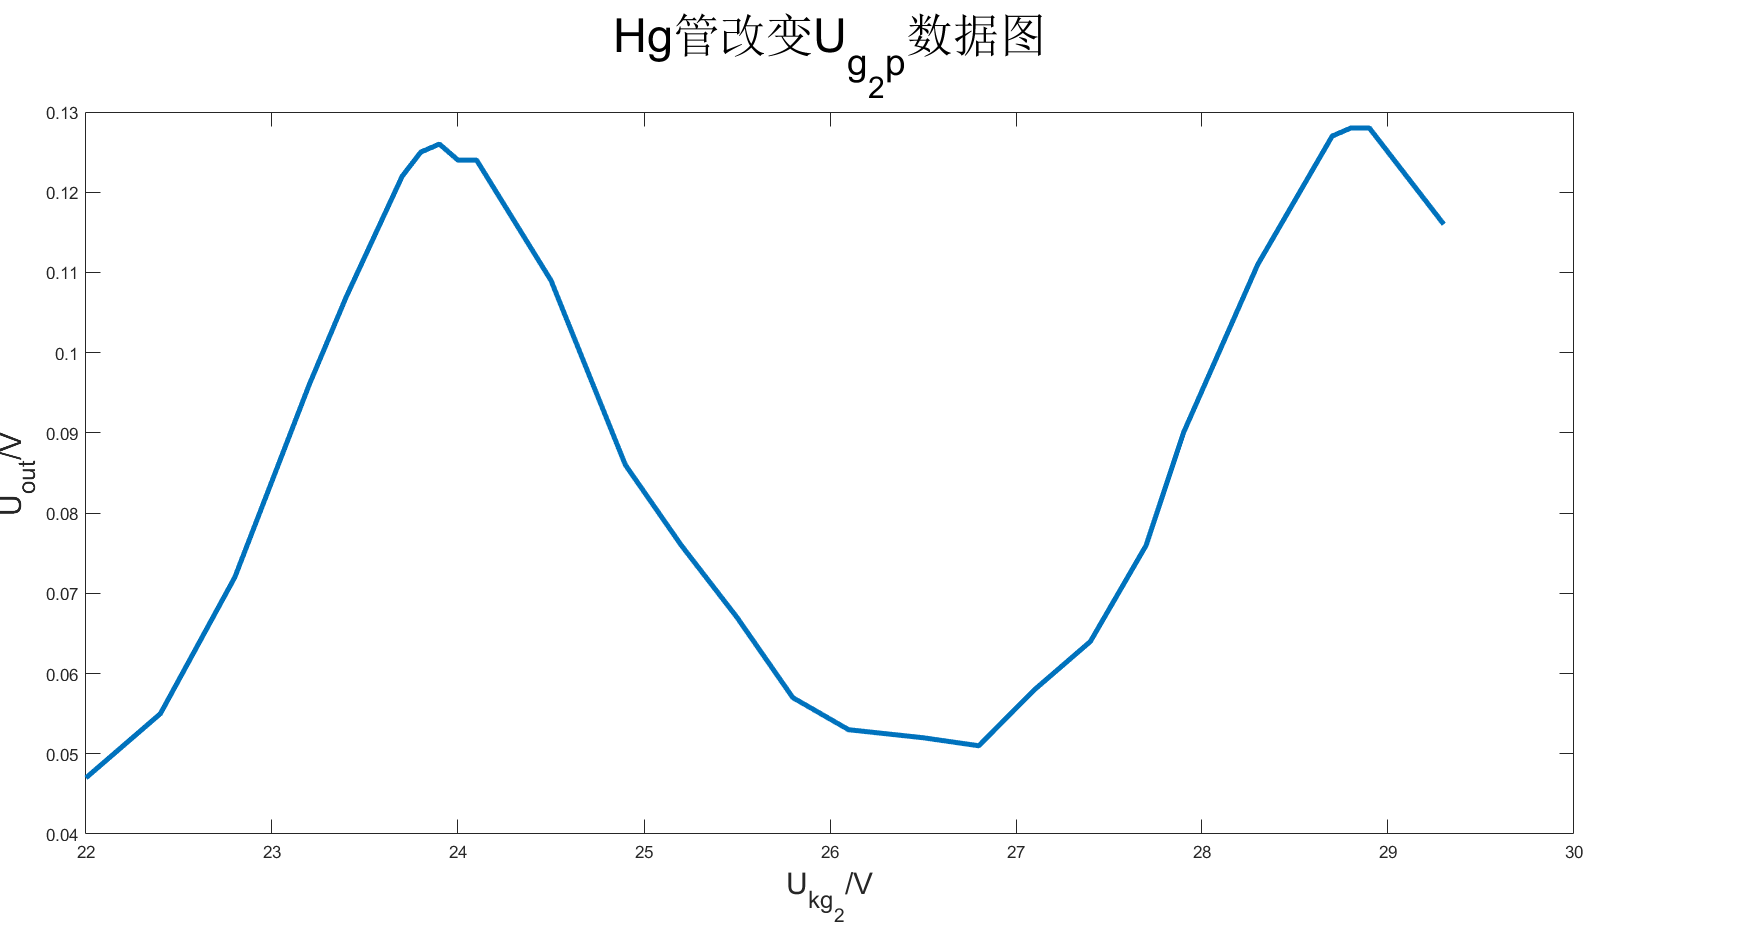
\includegraphics[width=18cm]{Hg2.92.png}}
\end{figure}

\subsubsection*{4.各峰值扫描电压}
\textcircled{1}Hg管数据如下:
\begin{table}[htbp]
\centering
\scalebox{1.5}{
\begin{tabular}{ccccccc}
\hline\hline
$n$&1&2&3&4&5&6 \\
\hline
$U_{kg_2}/V$&4.6&9.0&13.8&18.6&23.8&28.9 \\
\hline
\end{tabular}}
\end{table}
\par
设$U_{kg_2}=U_1*n+b$,其中的$U_1$即是Hg的第一激发电位.现在利用matlab使用最小二乘法进行运算,得出图(a).
\par
并且计算出$U_1=4.8771(V)$,且由$\dfrac{\sigma_{U_1}}{U_1}=\sqrt{\dfrac{1/r^2-1}{n-2}}$的公式得$\sigma_{U_1}=U_1\times \sqrt{\dfrac{1/r^2-1}{n-2}} $.则$\sigma_{U_1}=4.8771\times \dfrac{1}{2}\times \sqrt{1/(0.9996)^2-1}=0.06899\approx0.07(V)$,最后得出$U_1=(4.88\pm0.07)V$,或者表述为$U_1=(4.9\pm0.1)V$.
\par
\textcircled{2}Ar管数据如下:
\begin{table}[htbp]
\centering
\scalebox{1.5}{
\begin{tabular}{ccccccc}
\hline\hline
$n$&1&2&3&4&5&6 \\
\hline
$U_{kg_2}/V$&13.8&27.1&39.3&51.9&65.0&78.8 \\
\hline
\end{tabular}}
\end{table}
\par
设$U_{kg_2}=U_1*n+b$,其中的$U_1$即是Ar的第一激发电位.现在利用matlab使用最小二乘法进行运算,得出图(b).
\par
并且计算出$U_1=12.8943(V)$,且由$\dfrac{\sigma_{U_1}}{U_1}=\sqrt{\dfrac{1/r^2-1}{n-2}}$的公式得$\sigma_{U_1}=U_1\times \sqrt{\dfrac{1/r^2-1}{n-2}} $.则$\sigma_{U_1}=12.8943\times \dfrac{1}{2}\times \sqrt{1/(0.9998)^2-1}=0.12896\approx0.13(V)$,最后得出$U_1=(12.89\pm0.13)V$.\par
图(a)为:
\begin{figure}[htbp]
		\center{
		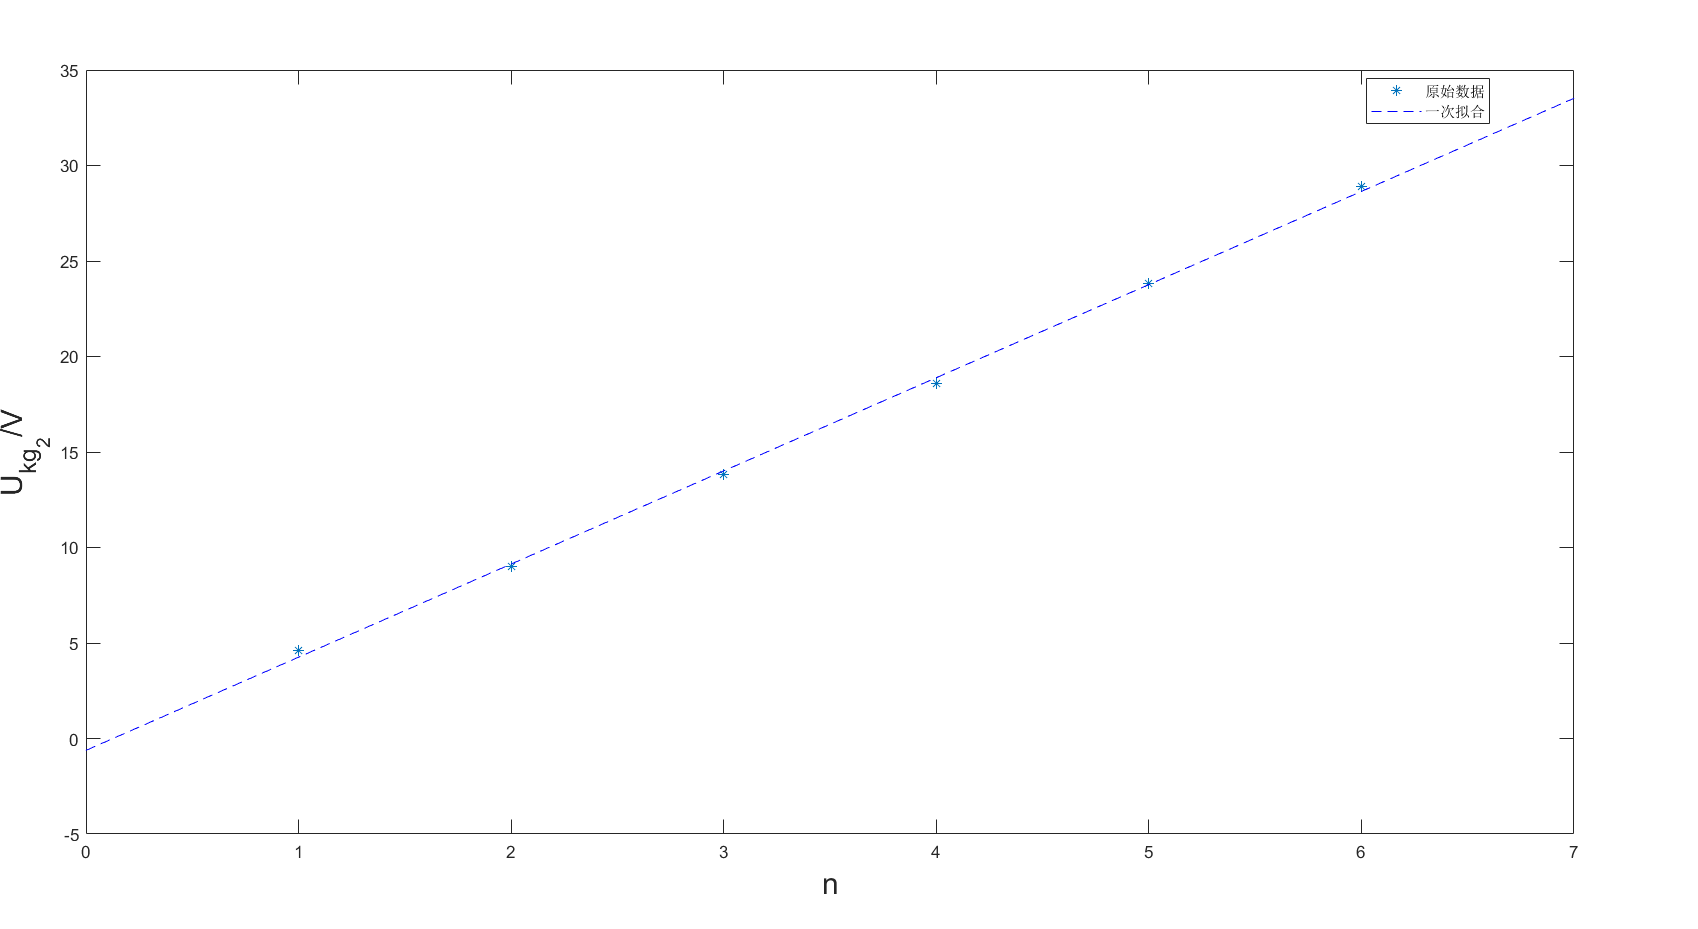
\includegraphics[width=15cm]{huigui1.png}}
	\end{figure}
	\par
	图(b)为:
	\begin{figure}[htbp]
	\center{
	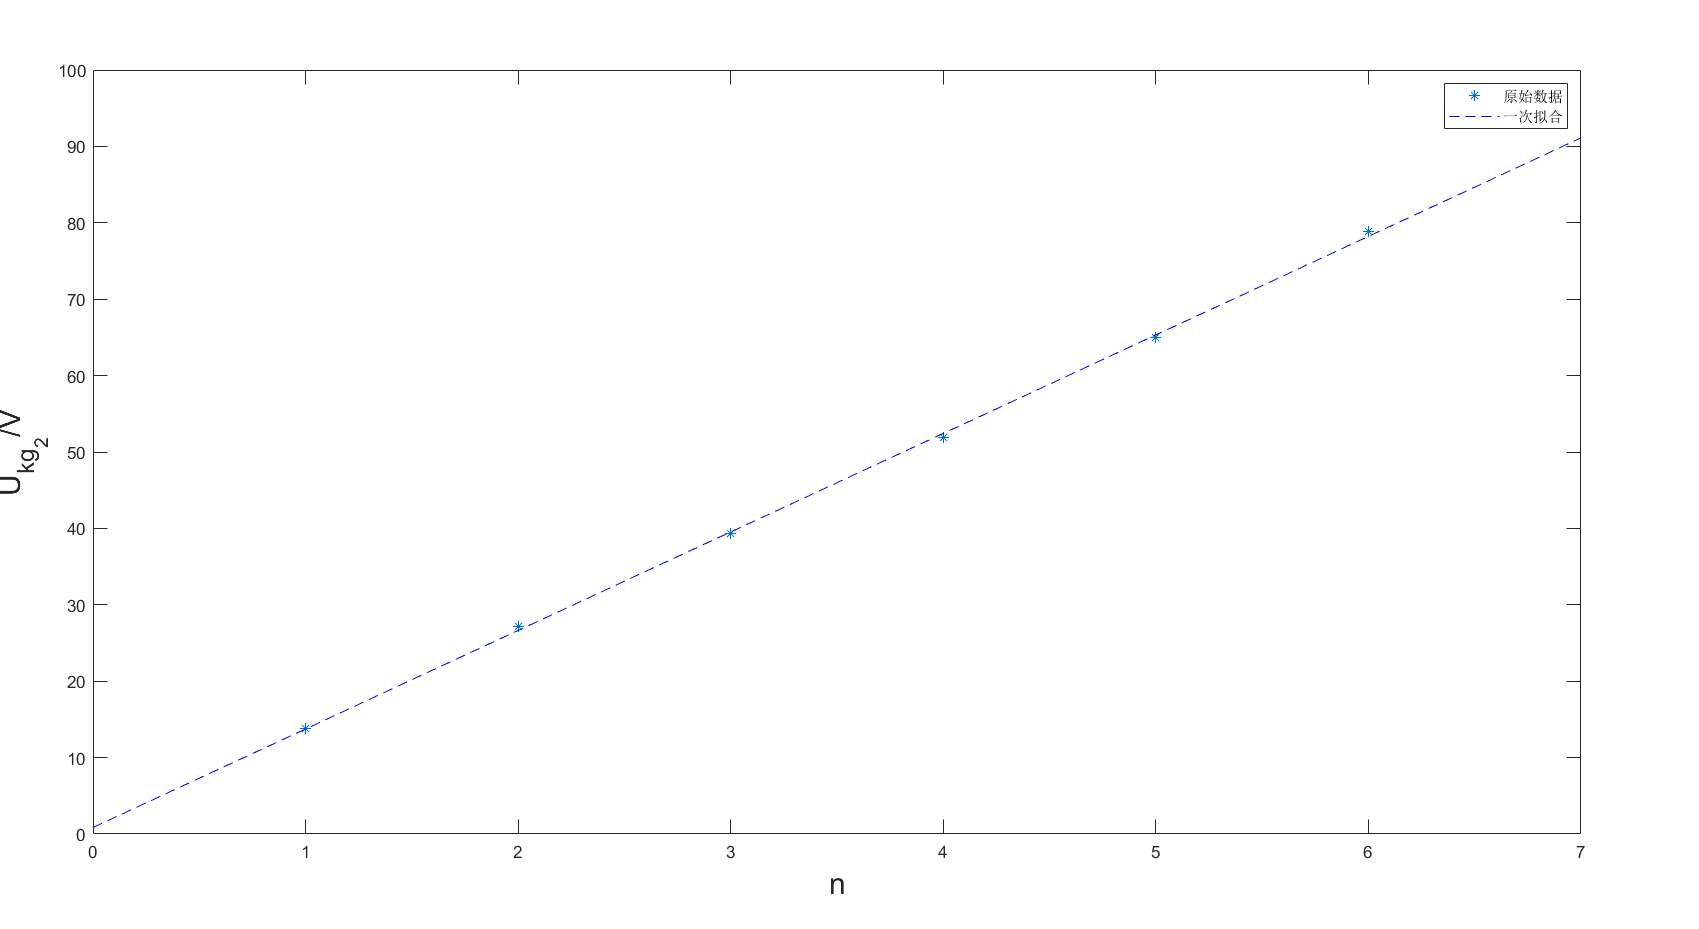
\includegraphics[width=15cm]{huigui2.png}}
	\end{figure}
\subsection*{【思考题】}
\textcircled{1}改变减速电压$U_{g_2p}$对曲线有何影响?\par
答:根据实验数据,当$U_{g_2p}=0.89V$时,峰高增加,峰位朝左方偏移,这是因为减速电压小了之后,电子达到极板时所需要的加速电压相对应地也变小了也有更多的电子能达到极板;当$U_{g_2p}=2.92V$时,峰高降低,峰位朝右方偏移,这是因为减速电压加大之后,电子达到极板变得困难,因此需要更大的加速电压,同时达到极板的电子也减少了.因此可推测出,当减速电压增加,峰高降低,峰位右移,当减速电压减小,峰高增加,峰位左移.\par
\textcircled{2}改变炉温对曲线有何影响?\par
答:由于未做实验,故用理论分析回答.当炉温升高,Hg蒸汽中原子数目增加,平均自由程减小,电子与之碰撞的概率增加,损失能量也就更多,到达极板的电子就越少,导致曲线峰高降低,且由于电子碰撞概率增加,将Hg激发的概率减小,因此需要更大的加速电压,峰位右移.当炉温降低,依照前面的分析,曲线的峰高增加,峰位左移.
\subsection*{【分析与讨论】}
\begin{enumerate}[1.]
\item 实验中测得的各种曲线有什么主要特征?如何理解? \par
答:各种曲线都具有峰值点(谷值点)的周期性,这主要是印证了原子能级的量子化.只有当电子能量满足能级差的整数倍时,电子才会将能量给被轰击原子,导致电流下降,而峰值点就是电子携带能量为能极差整数倍的状态,则根据峰值点之间的关联就可以知道能级差的关系.
\item 分析测量第一激发电位时误差的主要来源.\par
答:\textcircled{1}由于电子仪器在测量时对周围环境的敏感性导致读数时产生了误差.\textcircled{2}仪器自身的误差,比如在测量Ar管时,在低电压情况下,电流很小.\textcircled{3}测量时,$U_{kg_2}$的取值不稳定可能导致误差,未等系统稳定就测量也可能导致误差.
\end{enumerate}

\end{document}